\begin{custom-simple}[Problem 19]
\textbf{(a)} Since the lens is focused on infinity, we see that the groups of parallel arrays will focus onto the sensor. 
\begin{center}
    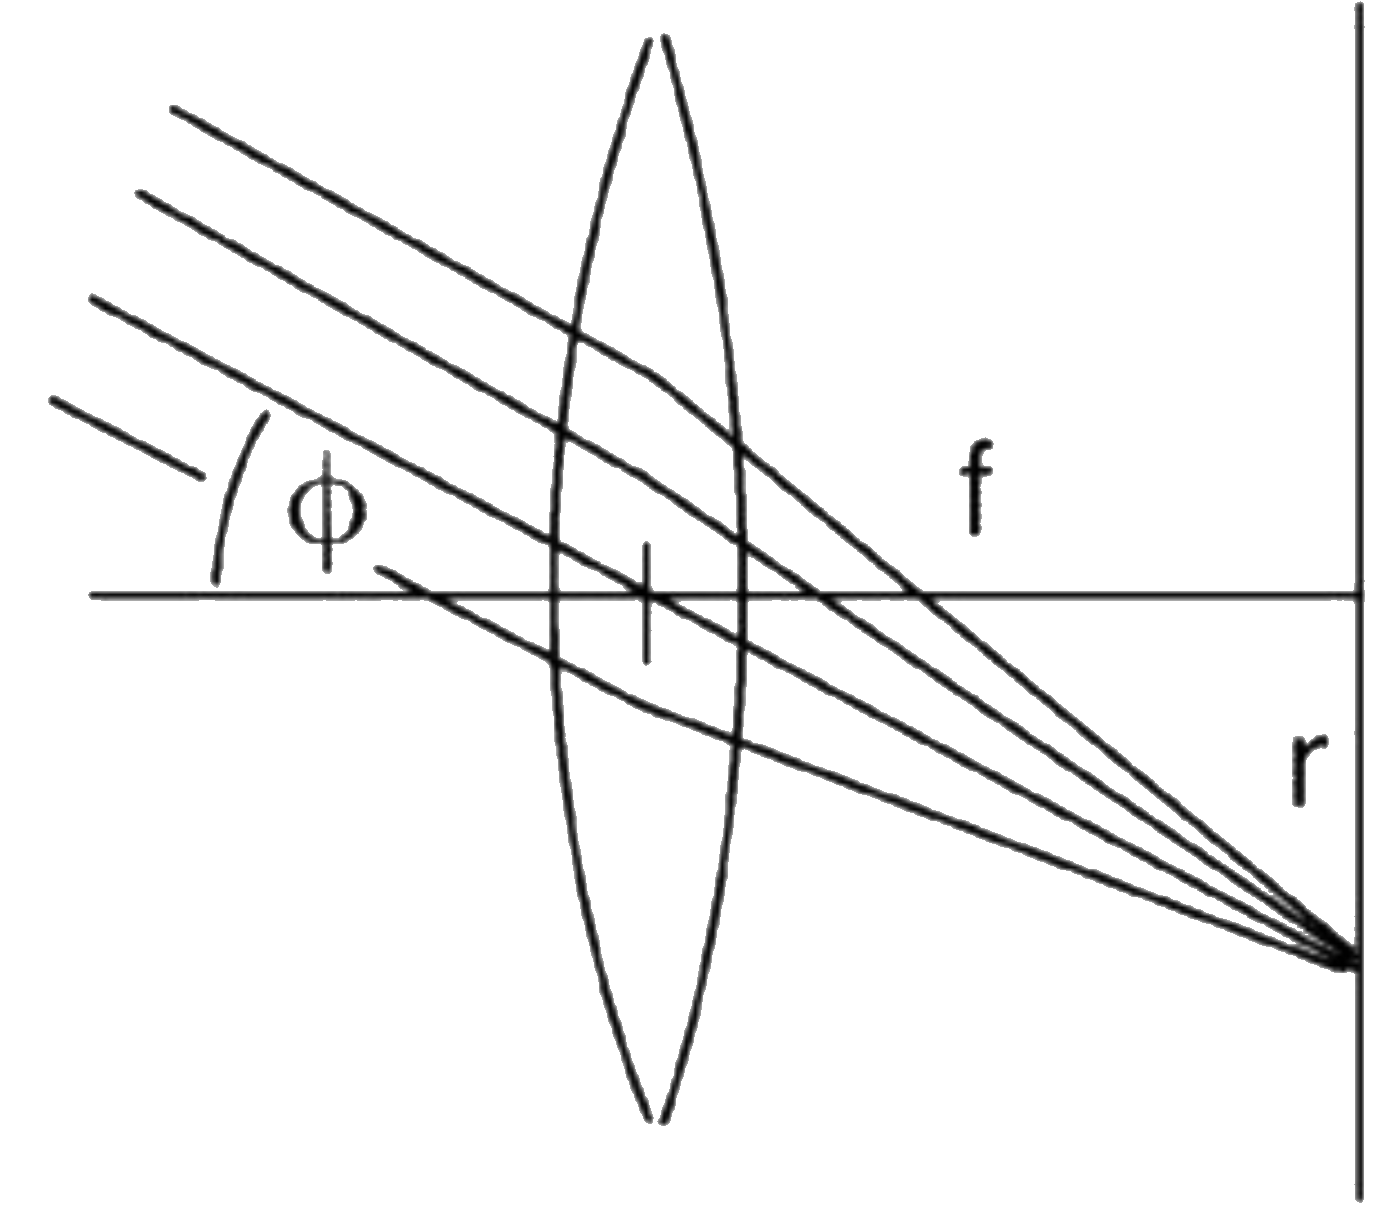
\includegraphics[width=0.5\linewidth]{kalda-physics-cup.png}
\end{center}
\vspace{5mm}
If the first minimum of the interference pattern focuses a distance $r$ away, then 
\[\frac{d}{2}\sin\phi = \frac{\lambda}{2}\]
where $d$ is the total width of the group of light rays. In small angle approximations, we see that 
\[\tan\phi \approx \sin\phi \implies \sin\phi \approx \frac{r}{f}.\]
Going back to our original expression, we see that 
\[\frac{d}{2}\frac{r}{f} = \frac{\lambda}{2}\implies d = \boxed{\frac{d\lambda}{r}}.\]

\textbf{(b)} There are several strange things about the picture on the paper:
\begin{itemize}
\item its colour is different—it is definitely not 404 nm violet, more like bluish white, longer wavelength;
\item it is much brighter (could be explained by the better sensitivity of the camera to longer wavelengths, see above);
\item it is ‘smoother’—mainly in that speckles are not visible in it.
\end{itemize}
As long as there is light scattered off a surface, there should be speckles visible in the picture. The lack of these could be explained by an insufficient resolution, but that does not seem right: the speckle size S'measured for other images was much larger than the pixel size. Also, when light is scattered, its wavelength does not change (unlike what was observed). Therefore, the only possible answer is: it is not a photograph of the scattered laser light, but a photograph of some other light that is created within the paper by the laser light.
\vspace{3mm}

This can only be a fluorescent light created when a light of a suitable wavelength is absorbed by a molecule. Then, an electron is excited to a higher energy level, and later returns to a lower level while emitting a photon. This explains the observed change in wavelength. Paper often contains such fluorescent molecules in low concentrations, because by absorbing UV light and emitting visible light of a higher wavelength, they make the paper seem whiter to the human eye, which has low sensitivity to short wavelengths (digital cameras recognize colours in a similar way, to make the pictures more realistic). The time required for a single absorption–emission process is not constant, and the fluorescent molecules are often so complicated that there are many allowed transitions with similar energy difference, so there are various emission–absorption processes possible, and the emitted light wavelength is not constant. This means that the light generated at the bright spot is completely random—not coherent, not even monochromatic. Thus, every illuminated spot on the paper acts like an independent (non-coherent) point source, and therefore no speckles form.
\vspace{3mm}

The camera is much more sensitive to a blue light than to a violet one. Therefore, even if some of the light from the bright spot is a scattered laser light which gives rise to weak speckles, these are not bright enough to be detected by the sensor. In the wall, however, fluorescence is negligible, so speckles which arise from random reflection from the wall can be seen.
\blfootnote{This solution is taken from the official 2012 Physics Cup Solution as it is much better at explaining things than us.}
\end{custom-simple}